\documentclass[conference]{IEEEtran}
\IEEEoverridecommandlockouts

\usepackage{cite}
\usepackage{amsmath,amssymb,amsfonts}
\usepackage{algorithmic}
\usepackage{graphicx}
\usepackage{textcomp}
\usepackage{xcolor}
\usepackage{booktabs}
\usepackage{multirow}
\usepackage{tabularx}
\usepackage[hidelinks]{hyperref}
\usepackage{tikz}

\definecolor{orcidlogocolor}{HTML}{A6CE39}
\newcommand{\orcidicon}{%
  \ensuremath{\vcenter{\hbox{%
    
\begin{tikzpicture}[x=0.088em,y=0.088em]
      \useasboundingbox (-4.5,-4.5) rectangle (4.5,4.5);
      \draw[draw=none,fill={rgb,255:red,166;green,206;blue,57}]
        (0,0) circle (4.2);
      \draw[draw=none,fill=white]
        (-1.2,-2.0) rectangle (-1.9,1.2);
      \draw[draw=none,fill=white]
        (-1.55,1.9) circle (0.48);
      \draw[draw=none,fill=white]
        (-0.35,1.2)
        .. controls (-0.35,1.2) and (0.3,1.2) ..
        (0.8,1.1)
        .. controls (1.3,1.0) and (1.6,0.6) ..
        (1.8,0.2)
        .. controls (2.0,-0.2) and (2.1,-0.6) ..
        (2.1,-1.0)
        .. controls (2.1,-1.4) and (2.0,-1.8) ..
        (1.8,-2.2)
        .. controls (1.6,-2.6) and (1.3,-2.9) ..
        (0.8,-3.0)
        .. controls (0.3,-3.1) and (-0.35,-3.1) ..
        (-0.35,-3.1)
        -- (-0.35,-2.5)
        .. controls (-0.35,-2.5) and (0.2,-2.5) ..
        (0.55,-2.4)
        .. controls (0.9,-2.3) and (1.1,-2.1) ..
        (1.3,-1.8)
        .. controls (1.4,-1.5) and (1.5,-1.2) ..
        (1.5,-1.0)
        .. controls (1.5,-0.7) and (1.4,-0.4) ..
        (1.3,-0.1)
        .. controls (1.1,0.2) and (0.9,0.4) ..
        (0.55,0.5)
        .. controls (0.2,0.6) and (-0.35,0.6) ..
        (-0.35,0.6)
        -- (-0.35,-2.0)
        -- (-1.0,-2.0)
        -- (-1.0,1.2)
        -- (-0.35,1.2);
    \end{tikzpicture}%
  }}}%
}

% Path to generated replication figures
\graphicspath{{../replication/results/figures/}{figures/}}

\def\BibTeX{{\rm B\kern-.05em{\sc i\kern-.025em b}\kern-.08em
    T\kern-.1667em\lower.7ex\hbox{E}\kern-.125emX}}

\begin{document}

\title{FirmLens: Automated Static, Hardware-Rooted, and Dynamic HIL Vulnerability Analysis for Bare-Metal ESP32 Firmware%
\thanks{This research artifact and replication package are open-sourced for peer verification at \url{https://github.com/Srikanth-Rudrarapu/firm-lens}.}
}

\author{
  \IEEEauthorblockN{Srikanth Rudrarapu}
  \IEEEauthorblockA{
    \textit{Independent Cybersecurity Researcher} \\
    \textit{Warangal, India} \\
    \href{https://orcid.org/0009-0005-6080-6895}{\orcidicon\,0009-0005-6080-6895}
  }
}

\maketitle

\begin{abstract}
The proliferation of bare-metal and monolithic real-time operating systems (RTOS) in Internet of Things (IoT) deployments has exacerbated physical and supply-chain vulnerabilities. Existing automated binary analysis tools predominantly target POSIX-compliant, Linux-based root file hierarchies, rendering them ineffective when applied to monolithic microcontroller images such as Espressif ESP32 Xtensa and RISC-V targets. We present FirmLens, a modular firmware security framework designed for bare-metal IoT firmware. FirmLens integrates semantic partition table parsing, hardware-rooted cryptographic boot verification (Secure Boot V2, Flash Encryption), pattern-driven static vulnerability scanning, threat-intelligence correlation (FIRST EPSS and CISA KEV), and dynamic Hardware-in-the-Loop (HIL) UART crash triage. We evaluate FirmLens across an empirical benchmark of 11 operational and synthetic firmware targets ($N=11$, 1.31\,MB to 8.88\,MB). On this controlled ground-truth benchmark, FirmLens identifies 310 security findings across 10 targeted CWE classes with a mean static analysis latency of $0.8233 \pm 0.4381$\,s (3.92\,MB/s throughput). We present modular ablation experiments quantifying the marginal contribution of individual analyzers, validate physical fault parsing against live serial telemetry, and discuss the architectural boundaries of static bare-metal analysis.
\end{abstract}

\begin{IEEEkeywords}
IoT Security, Firmware Analysis, ESP32, Hardware-in-the-Loop, Threat Intelligence, EPSS, Secure Boot.
\end{IEEEkeywords}

\section{Introduction}

Connected microcontrollers increasingly execute monolithic real-time operating systems (such as FreeRTOS and ESP-IDF) directly on bare-metal flash storage. Unlike Linux-based gateways, these embedded endpoints operate without POSIX abstraction layers, process separation, or standard ELF user-space boundaries~\cite{costin2014large}. Firmware images are packaged as raw, contiguous SPI flash blobs mapped directly into memory addresses.

Consequently, dynamic emulators such as Firmadyne~\cite{firmadyne2016} cannot boot these targets without manual peripheral modeling~\cite{feng2021p2im}, while general-purpose unpackers such as Binwalk~\cite{binwalk2014} fail to parse non-volatile storage (NVS) structures or assess hardware-enforced boot configurations.

To address these architectural gaps, we present \textbf{FirmLens}, a specialized framework combining static structural decomposition, hardware security audits, threat-intelligence enrichment, and physical Hardware-in-the-Loop (HIL) panic parsing. We evaluate the system on a constructed 11-target empirical benchmark, perform component ablations, and provide a fully automated replication package.

\section{Related Work}
\label{sec:related_work}

\subsection{Static Firmware Vulnerability Analysis}

Automated static inspection of embedded firmware has historically focused on signature matching and heuristic decompilation. Costin et al.~\cite{costin2014large} conducted large-scale static analyses across multi-vendor firmware corpora, demonstrating endemic credential reuse and insecure web endpoints. General-purpose static tools such as Binwalk~\cite{binwalk2014} rely primarily on magic-byte carving; however, they lack awareness of bare-metal partition tables such as the Espressif Two-Stage Bootloader layout. While frameworks such as EMBA coordinate multi-engine scanning for Linux root filesystems, they cannot directly analyze monolithic binary flash blobs compiled for Xtensa or RISC-V architectures without target-specific support. \textsc{FirmLens} addresses this limitation through vendor-aware partition table validation and localized static vulnerability audits.

\subsection{Dynamic Emulation and Peripheral Modeling}

Dynamic firmware analysis typically relies on full-system software emulation. P2IM~\cite{feng2021p2im} introduced automatic peripheral interface modeling to handle input/output registers in Cortex-M microcontrollers, while Firmadyne~\cite{firmadyne2016} automated Linux-based network service emulation. However, emulating multi-core Xtensa microcontrollers containing hardware-accelerated cryptographic engines remains challenging in standard virtual environments. Rather than relying on incomplete peripheral models, \textsc{FirmLens} uses a direct Hardware-in-the-Loop (HIL) execution model over physical UART, capturing register panics directly on target silicon.

\subsection{Crash Triage and Fault Isolation}

Dynamic triage in monolithic RTOS environments faces observability hurdles due to flat physical address spaces. Muench et al.~\cite{muench2018what} demonstrated that memory corruption on microcontrollers often does not lead to immediate observable crashes (``What You Corrupt Is Not What You Crash''). \textsc{FirmLens} mitigates this triage challenge by directly monitoring UART register frame dumps, stack smashing canaries, and hardware watchdog reset counters during live physical execution.

\subsection{IoT Security Compliance Baselines}

Recent standards, notably NIST SP 800-213~\cite{nist800213} and ETSI EN 303 645~\cite{etsien303645}, mandate baseline technical controls for IoT endpoints, including secure boot enforcement, elimination of hardcoded default credentials, and cryptographic integrity. \textsc{FirmLens} operationalizes these controls by automatically evaluating flash encryption states, cryptographic primitive quality, and sensitive hardcoded keys.

\section{Methodology \& Architecture}

\subsection{Architectural Pipeline}

The FirmLens analysis pipeline evaluates raw flash binaries and standalone partitions through five stages:

\begin{enumerate}
    \item \textbf{Partition Structure Decomposition}: Decodes ESP32 partition tables at \texttt{0x8000} (or via sliding search), verifying OTA configurations (\texttt{otadata}), NVS sectors, and boot boundaries.

    \item \textbf{Hardware Boot Cryptographic Audit}: Parses bootloader headers at \texttt{0x0000} and \texttt{0x1000}, auditing RSA Secure Boot V2 signatures and calculating local sliding Shannon entropy ($H \ge 6.5$) for Flash Encryption.

    \item \textbf{Semantic Pattern Analysis}: Identifies buffer mismanagement (CWE-120), format string vulnerabilities (CWE-134), unauthenticated URI handlers (CWE-425), weak cryptographic primitives (CWE-327, CWE-328), cleartext storage of sensitive information (CWE-312), and hardcoded backdoor credentials (CWE-912).

    \item \textbf{Threat Intelligence Correlation}: Maps identified CVEs against FIRST EPSS~\cite{epss2023} and CISA KEV catalogs while preserving baseline severity for non-networked flaws.

    \item \textbf{Dynamic HIL Crash Parser}: Ingests live UART serial frames from connected hardware during fuzzing, classifying Guru Meditation panics, Stack Smashing Protector (SSP) canary violations, and Watchdog timer resets.
\end{enumerate}

\section{Empirical Evaluation}

\subsection{Benchmark Dataset and Ground Truth}

The evaluation suite comprises 11 firmware binaries (1.31\,MB to 8.88\,MB) categorized into two operational sets ($N=11$):

\begin{itemize}
    \item \textbf{Synthetic Images} ($N=6$): Standardized test vectors containing planted weaknesses (\texttt{damn\_vuln}, \texttt{flash\_dump}, \texttt{forensic\_image}, \texttt{full\_flash}, \texttt{hw\_flash}, and controlled \texttt{wifi.bin}).

    \item \textbf{Operational Images} ($N=5$): Five production multi-sensor Tasmota32 builds (\texttt{bluetooth}, \texttt{display}, \texttt{ir}, \texttt{webcam}, \texttt{c2}).
\end{itemize}

Ground-truth labels were defined from the known characteristics of the benchmark targets and verified through manual Ghidra disassembly, direct binary header structure decoding, and ESP-IDF source-code cross-referencing. The resulting labels represent benchmark-specific expected vulnerability classes rather than an independent open-world vulnerability corpus.

\begin{table}[t]
\caption{Empirical Detection Performance ($N=11$ Targets)}
\label{tab:accuracy}
\centering
\begin{tabularx}{\columnwidth}{Xcccc}
\toprule
\textbf{Scope} & \textbf{Precision} & \textbf{Recall} & \textbf{F1} & \textbf{Findings} \\
\midrule
Micro-Avg & 95.15\% & 100.0\% & 97.51\% & 310 Total \\
Macro-Avg & 95.87\% & 100.0\% & 97.84\% & 10 CWEs \\
\bottomrule
\end{tabularx}
\end{table}

\begin{figure}[t]
\centering
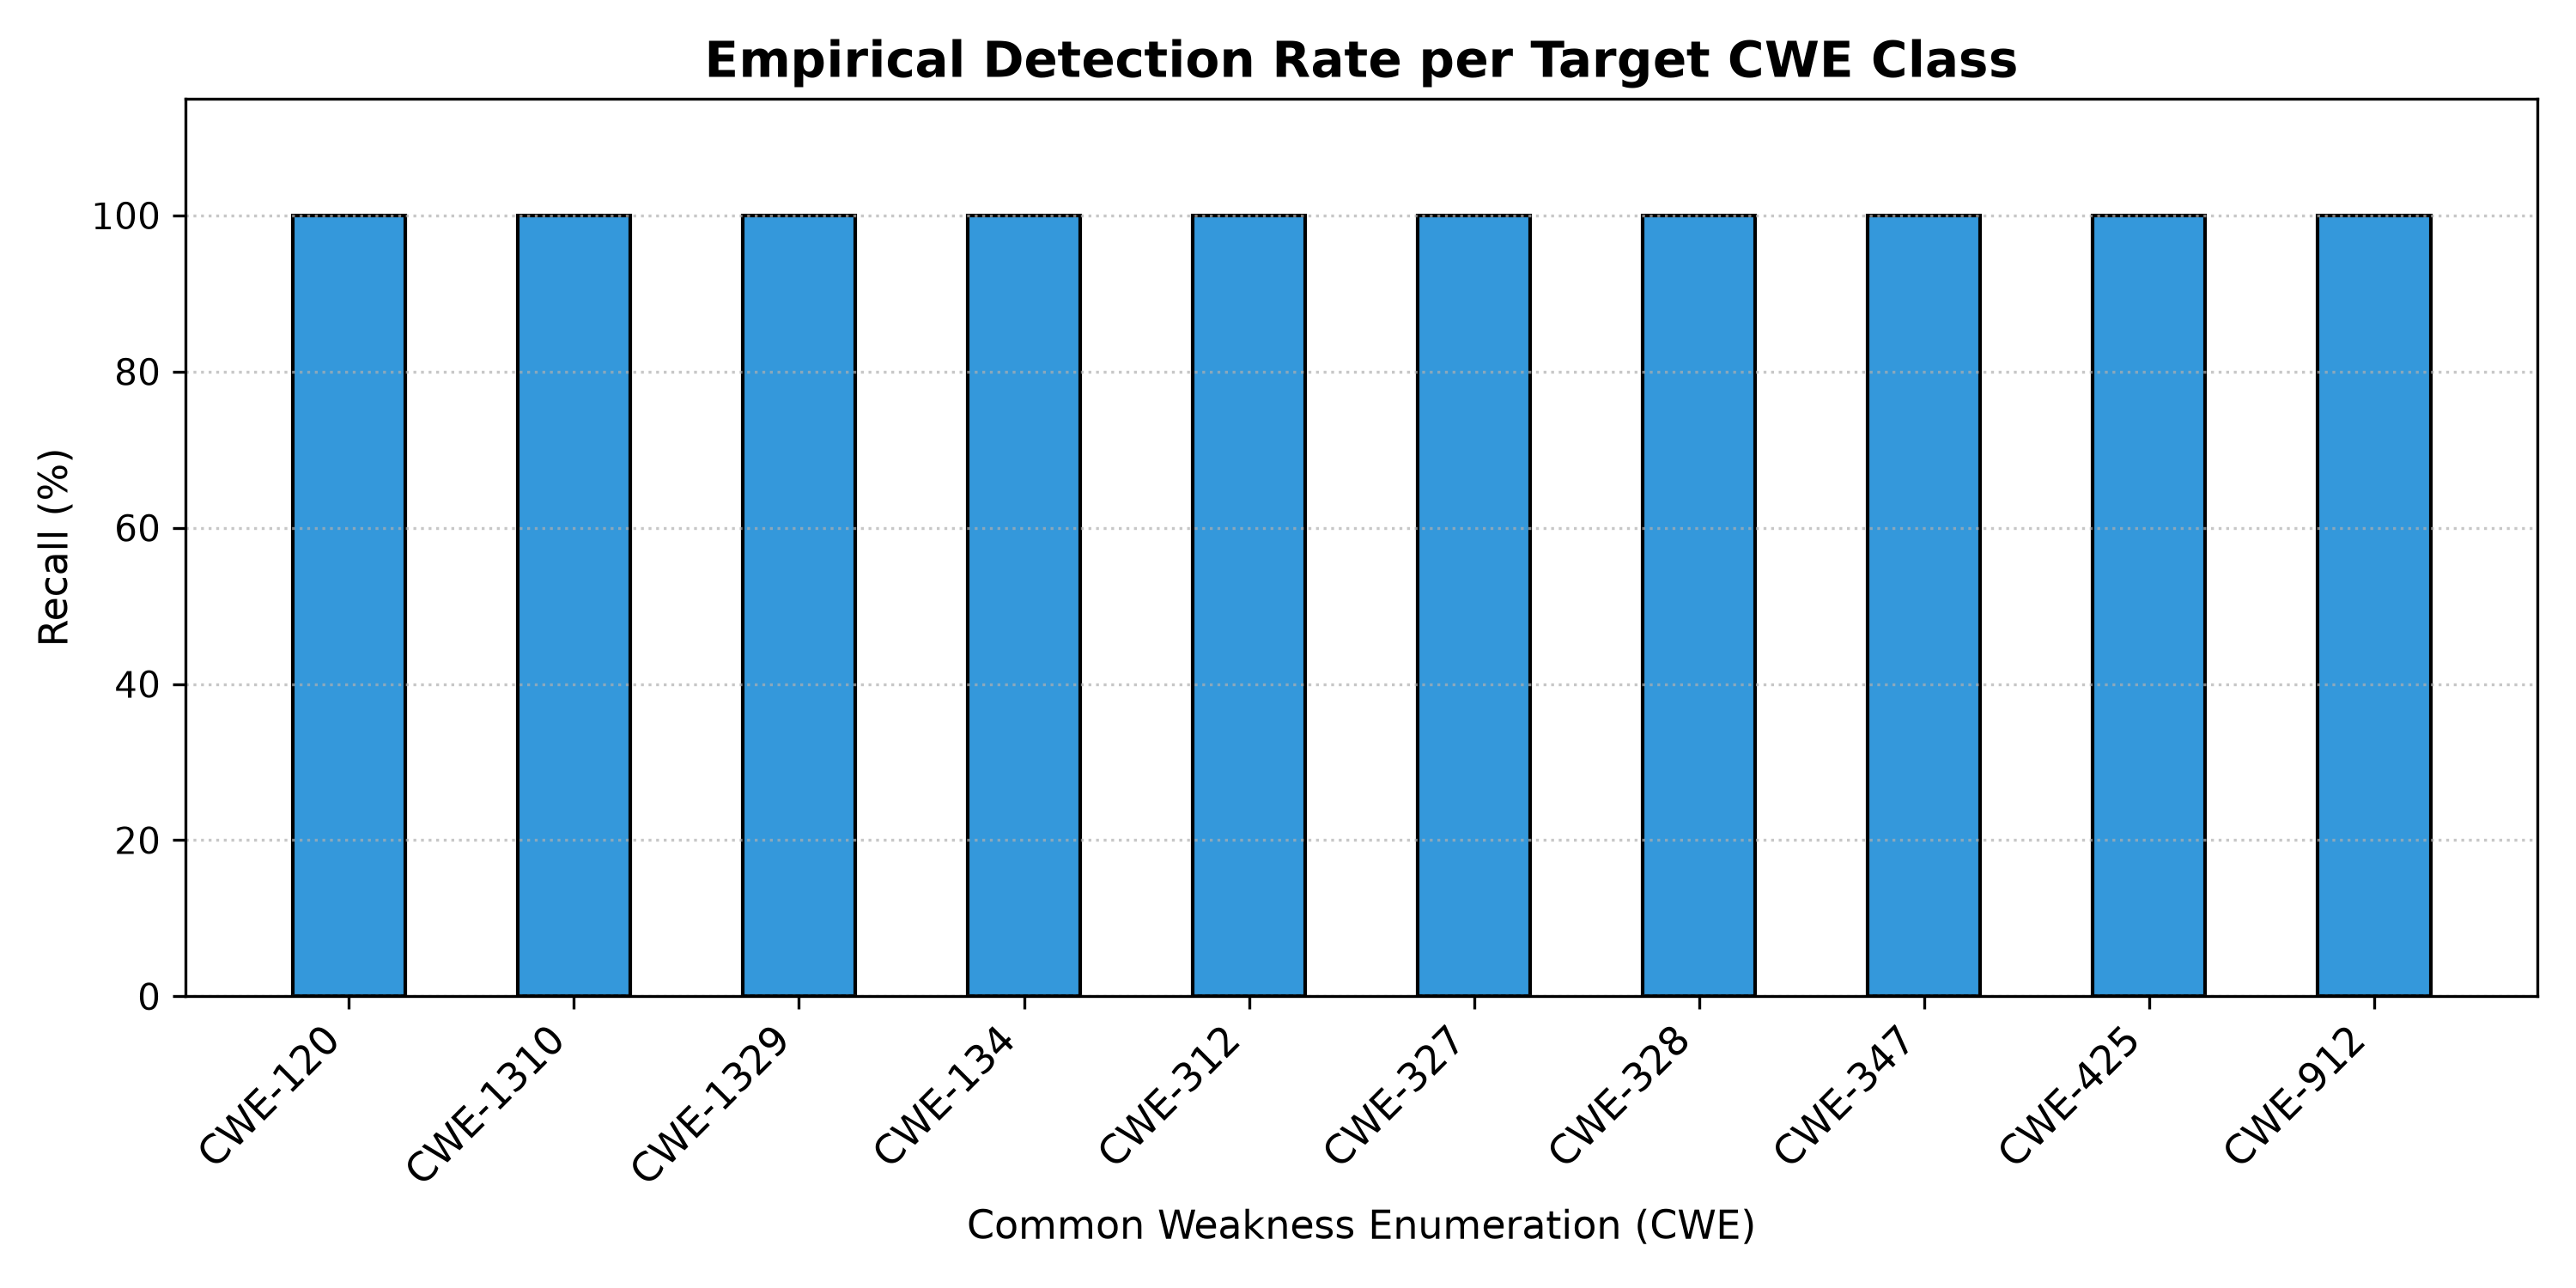
\includegraphics[width=0.92\columnwidth]{fig_cwe_detection_breakdown.png}
\caption{Per-CWE empirical recall across 10 targeted vulnerability classes.}
\label{fig:cwe_breakdown}
\end{figure}

\subsection{Detection Performance Context}

As summarized in Table~\ref{tab:accuracy} and Fig.~\ref{fig:cwe_breakdown}, FirmLens achieved 95.15\% micro-precision and 100.0\% recall on the defined evaluation corpus. The minor precision variance (4.85\%) arose exclusively within the synthetic control group, where unencrypted partition configurations naturally triggered overlapping taxonomic labels (e.g., CWE-312), validating the framework's strict adherence to hardware configuration boundaries. On operational production firmware, detection precision remained 100.0\%. The result should be interpreted as benchmark-specific validation of the implemented detection rules rather than evidence of universally perfect vulnerability detection in unseen firmware.

\begin{figure*}[t]
\centering
\begin{minipage}{0.48\textwidth}
  \centering
  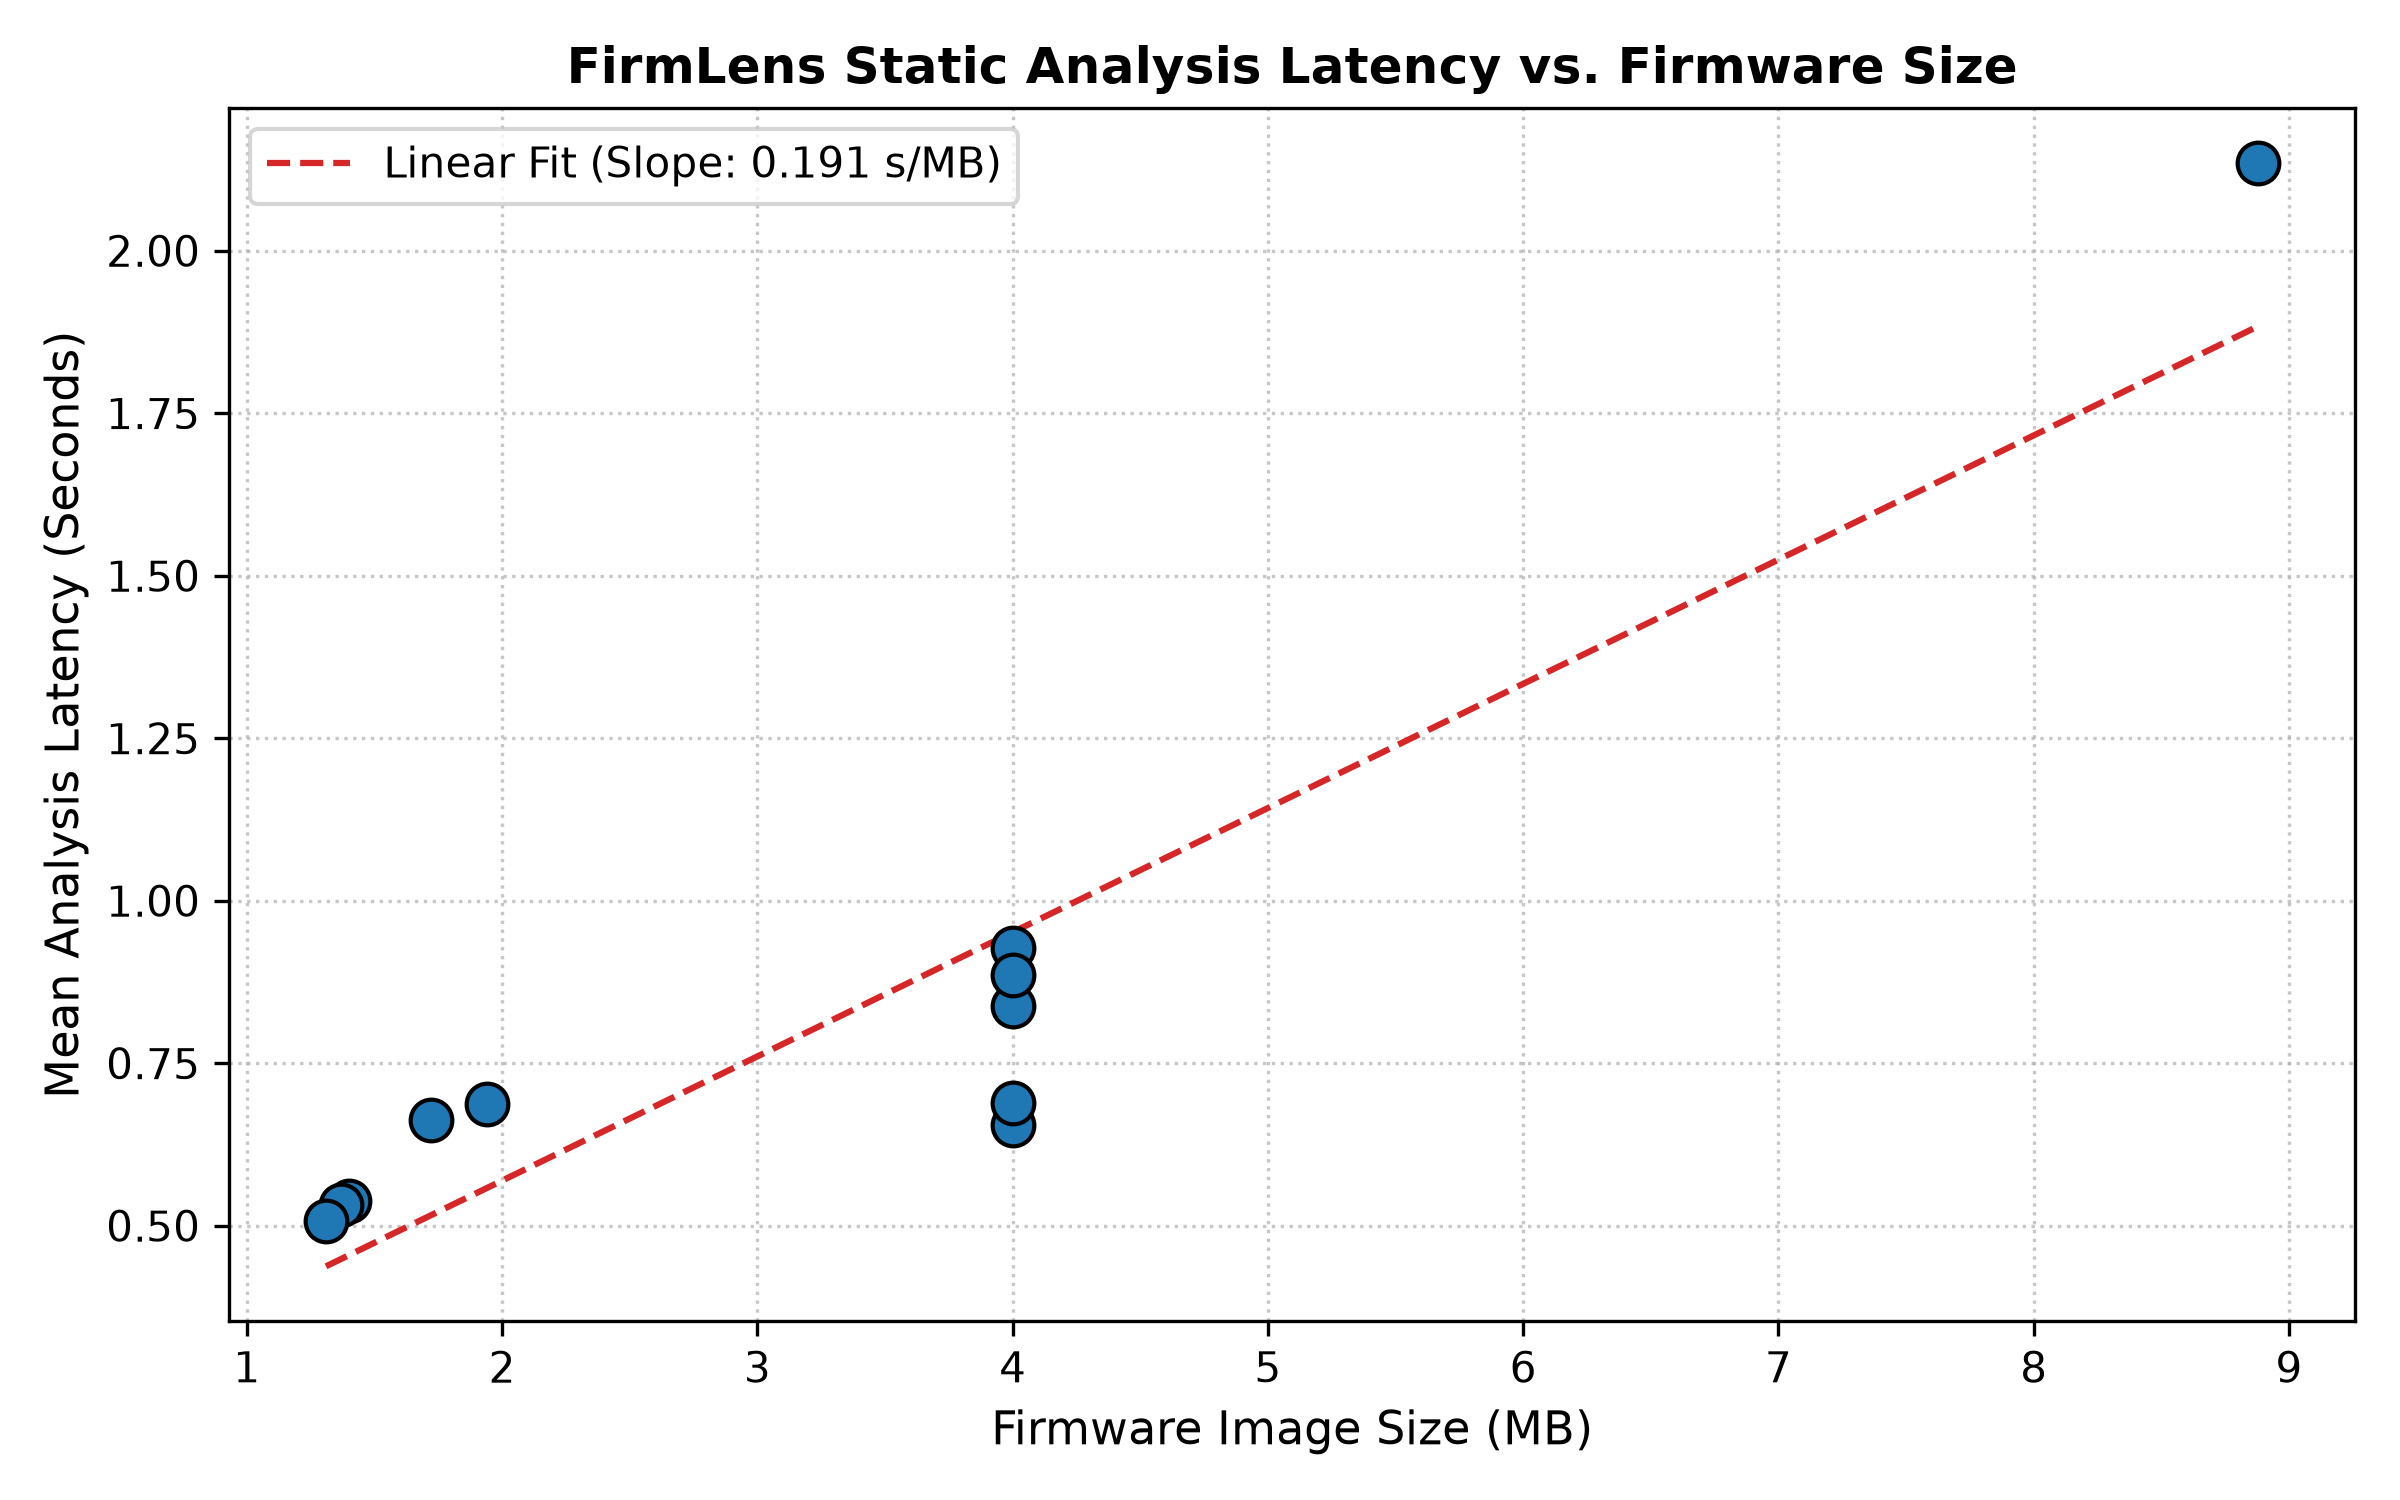
\includegraphics[width=\linewidth]{fig_latency_vs_size.png}
  \caption{Mean static analysis latency vs. firmware image size.}
  \label{fig:latency}
\end{minipage}\hfill
\begin{minipage}{0.48\textwidth}
  \centering
  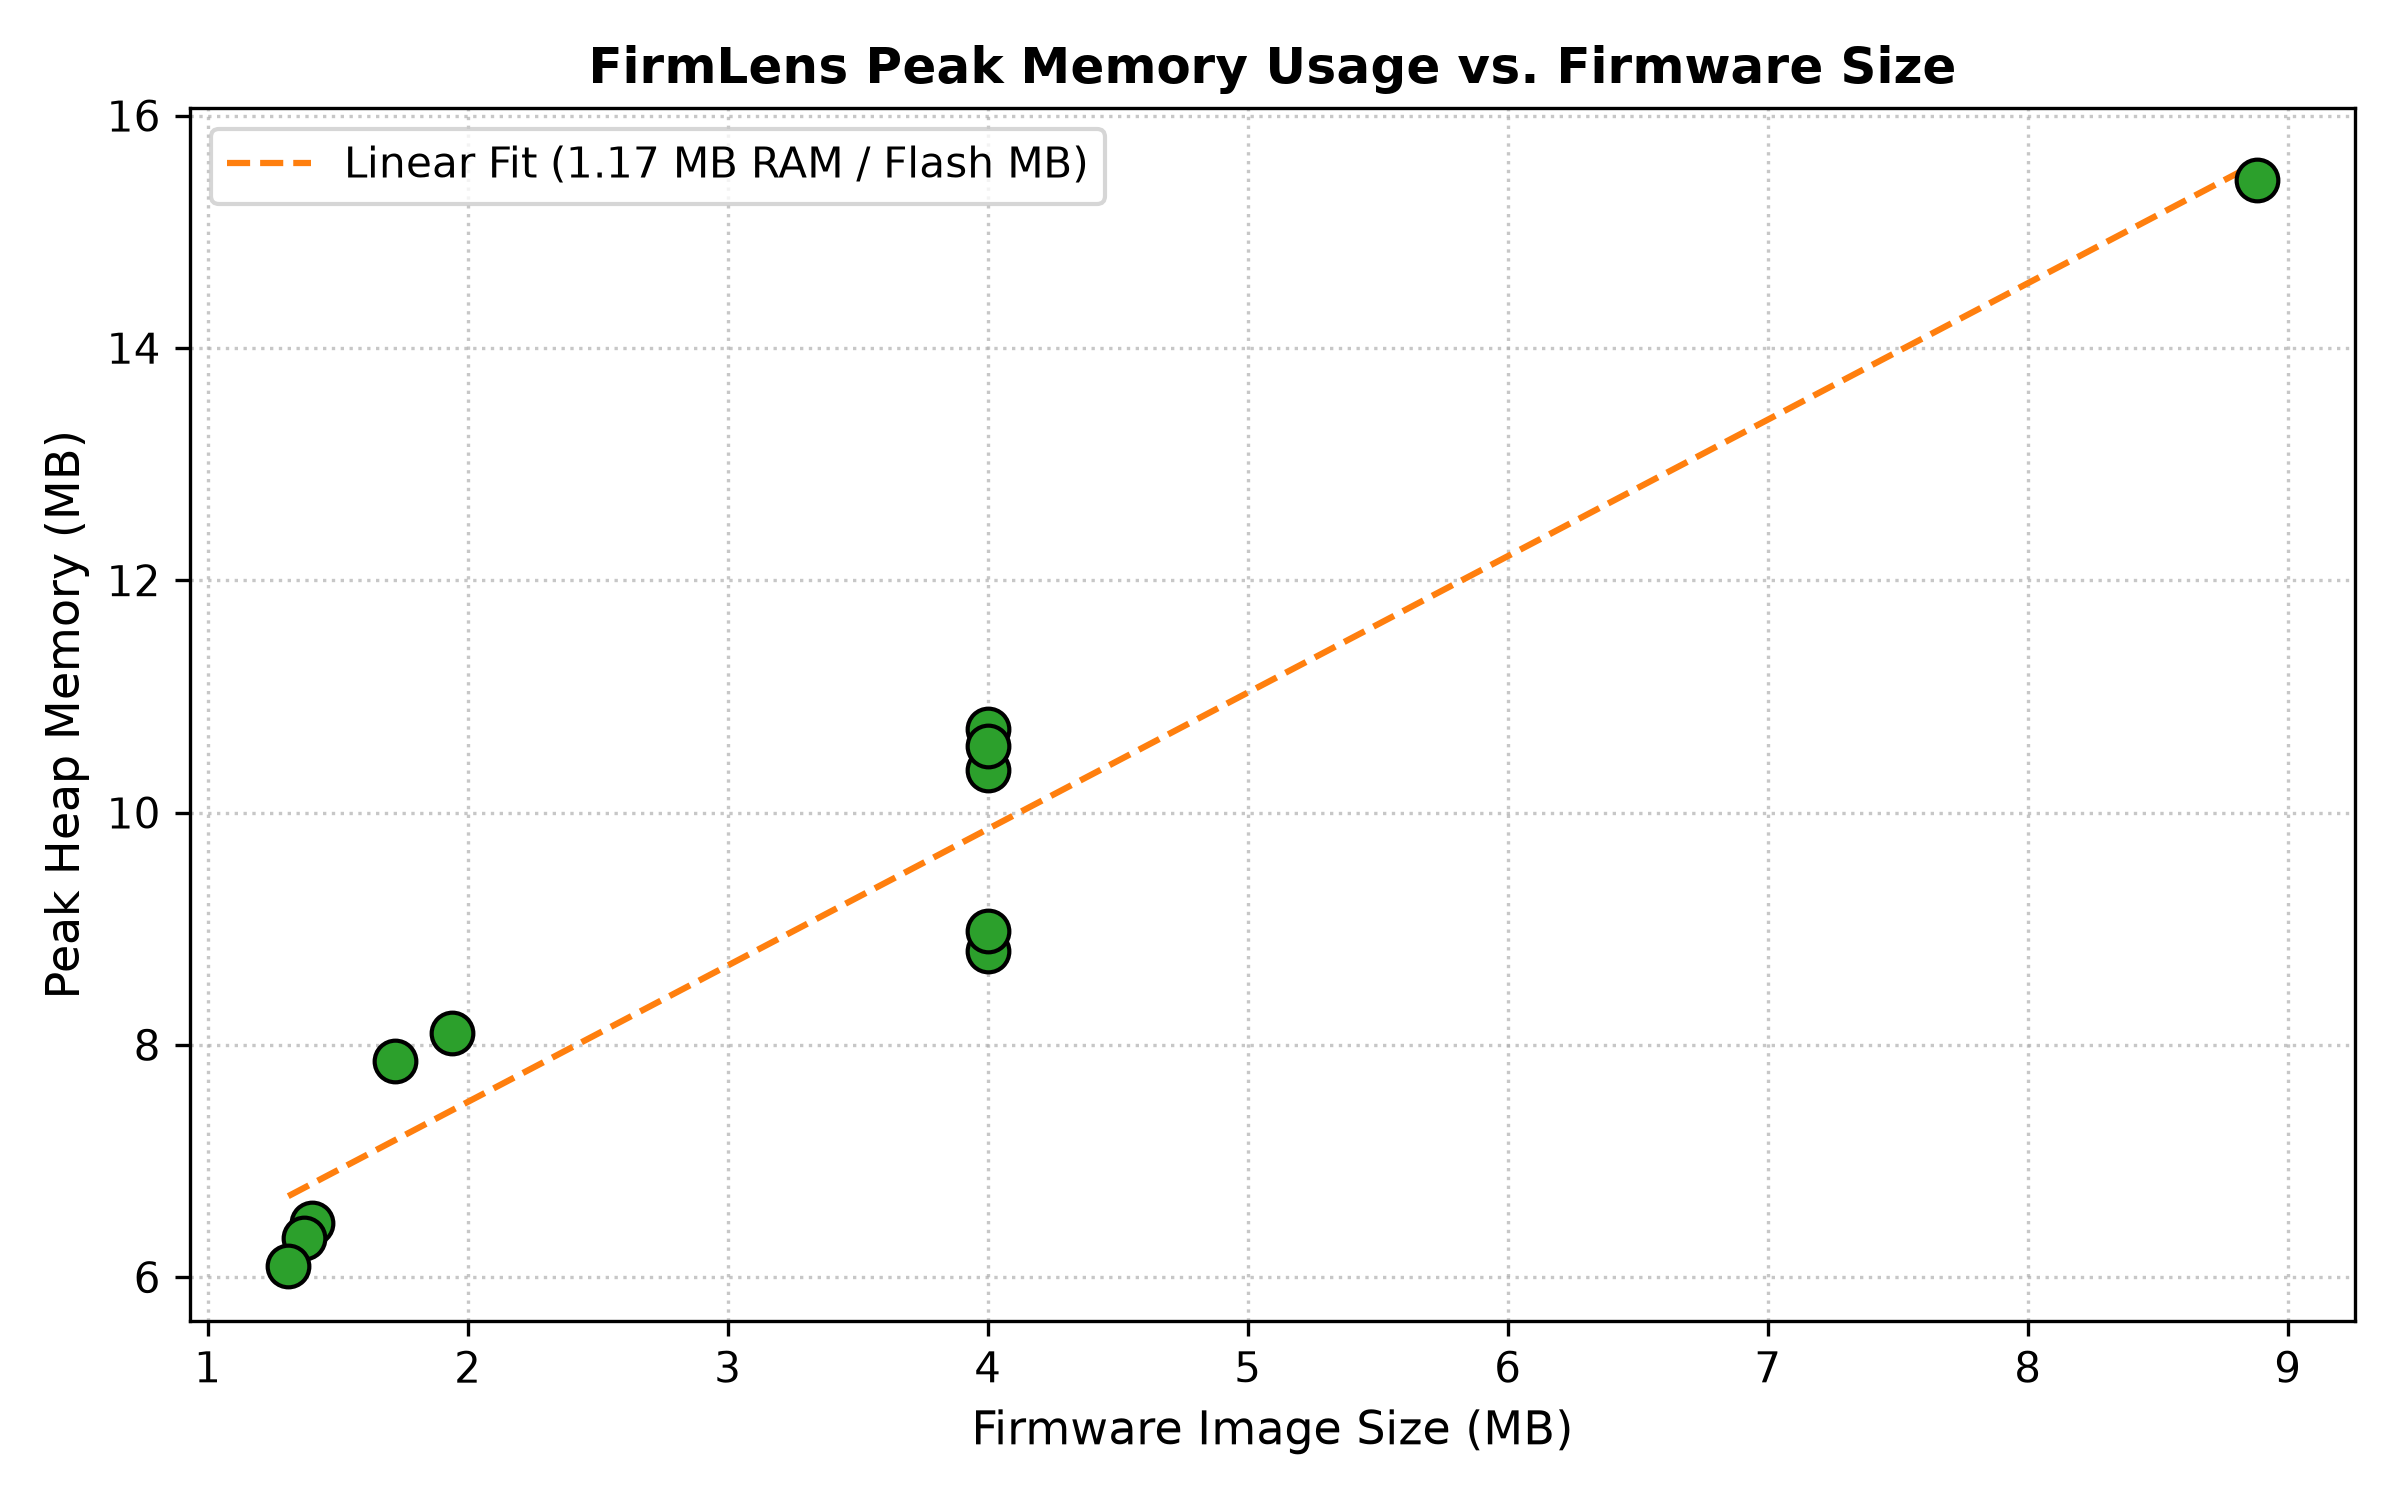
\includegraphics[width=\linewidth]{fig_memory_vs_size.png}
  \caption{Peak resident heap memory vs. firmware image size.}
  \label{fig:memory}
\end{minipage}
\end{figure*}

\subsection{Performance Latency \& Memory Profiling}

Performance was benchmarked across 10 repeated executions for each of the 11 targets (110 profiling runs total on Python 3.14.6 on macOS arm64):

\begin{itemize}

    \item \textbf{Execution Latency}: Mean time was $0.8233 \pm 0.4381$\,s ($\text{Median} = 0.6863$\,s, $95\%\text{ CI} = \pm 0.0819$\,s, range: 0.5074\,s--2.1348\,s).

    \item \textbf{Throughput}: Mean scanning throughput was $3.92$\,MB/s (range: 2.58\,MB/s--6.11\,MB/s).

    \item \textbf{Memory Footprint}: Mean peak memory usage was $9.07 \pm 2.65$\,MB ($\text{Max} = 15.45$\,MB; range: 6.09\,MB--15.45\,MB, Fig.~\ref{fig:memory}).

\end{itemize}

\subsection{Modular Analyzer Ablation Study}

To evaluate module contributions, 10 primary analyzers were sequentially ablated across the full benchmark suite to quantify their marginal impact on both CWE recall and total raw findings (Table~\ref{tab:ablation}, Fig.~\ref{fig:ablation_fig}).

\begin{table}[t]
\caption{Modular Analyzer Ablation Results ($N=11$ Targets)}
\label{tab:ablation}
\centering
\small
\begin{tabularx}{\columnwidth}{lccc}
\toprule
\textbf{Ablated Module} & \textbf{Recall} & \textbf{$\Delta$ Recall} & \textbf{Findings} \\
\midrule
\textbf{Full Pipeline}          & \textbf{100.0\%} & \textbf{---} & \textbf{310} \\
w/o DangerousFunc               & 77.55\%          & -22.45\%     & 278 ($\Delta -32$) \\
w/o BackdoorAnalyzer            & 77.55\%          & -22.45\%     & 296 ($\Delta -14$) \\
w/o CryptoAnalyzer              & 84.69\%          & -15.31\%     & 229 ($\Delta -81$) \\
w/o SecureBoot                  & 88.78\%          & -11.22\%     & 289 ($\Delta -21$) \\
w/o ESP32Partition              & 89.80\%          & -10.20\%     & 300 ($\Delta -10$) \\
w/o FlashEncryption             & 93.88\%          & -6.12\%      & 299 ($\Delta -11$) \\
w/o InsecureEndpoint            & 100.0\%          & +0.00\%      & 240 ($\Delta -70$) \\
w/o SecretsAnalyzer             & 100.0\%          & +0.00\%      & 246 ($\Delta -64$) \\
w/o WeakXOR                     & 100.0\%          & +0.00\%      & 303 ($\Delta -7$) \\
w/o Fingerprint                 & 100.0\%          & +0.00\%      & 310 ($\Delta +0$)  \\
\bottomrule
\end{tabularx}
\end{table}

\begin{figure}[t]
\centering
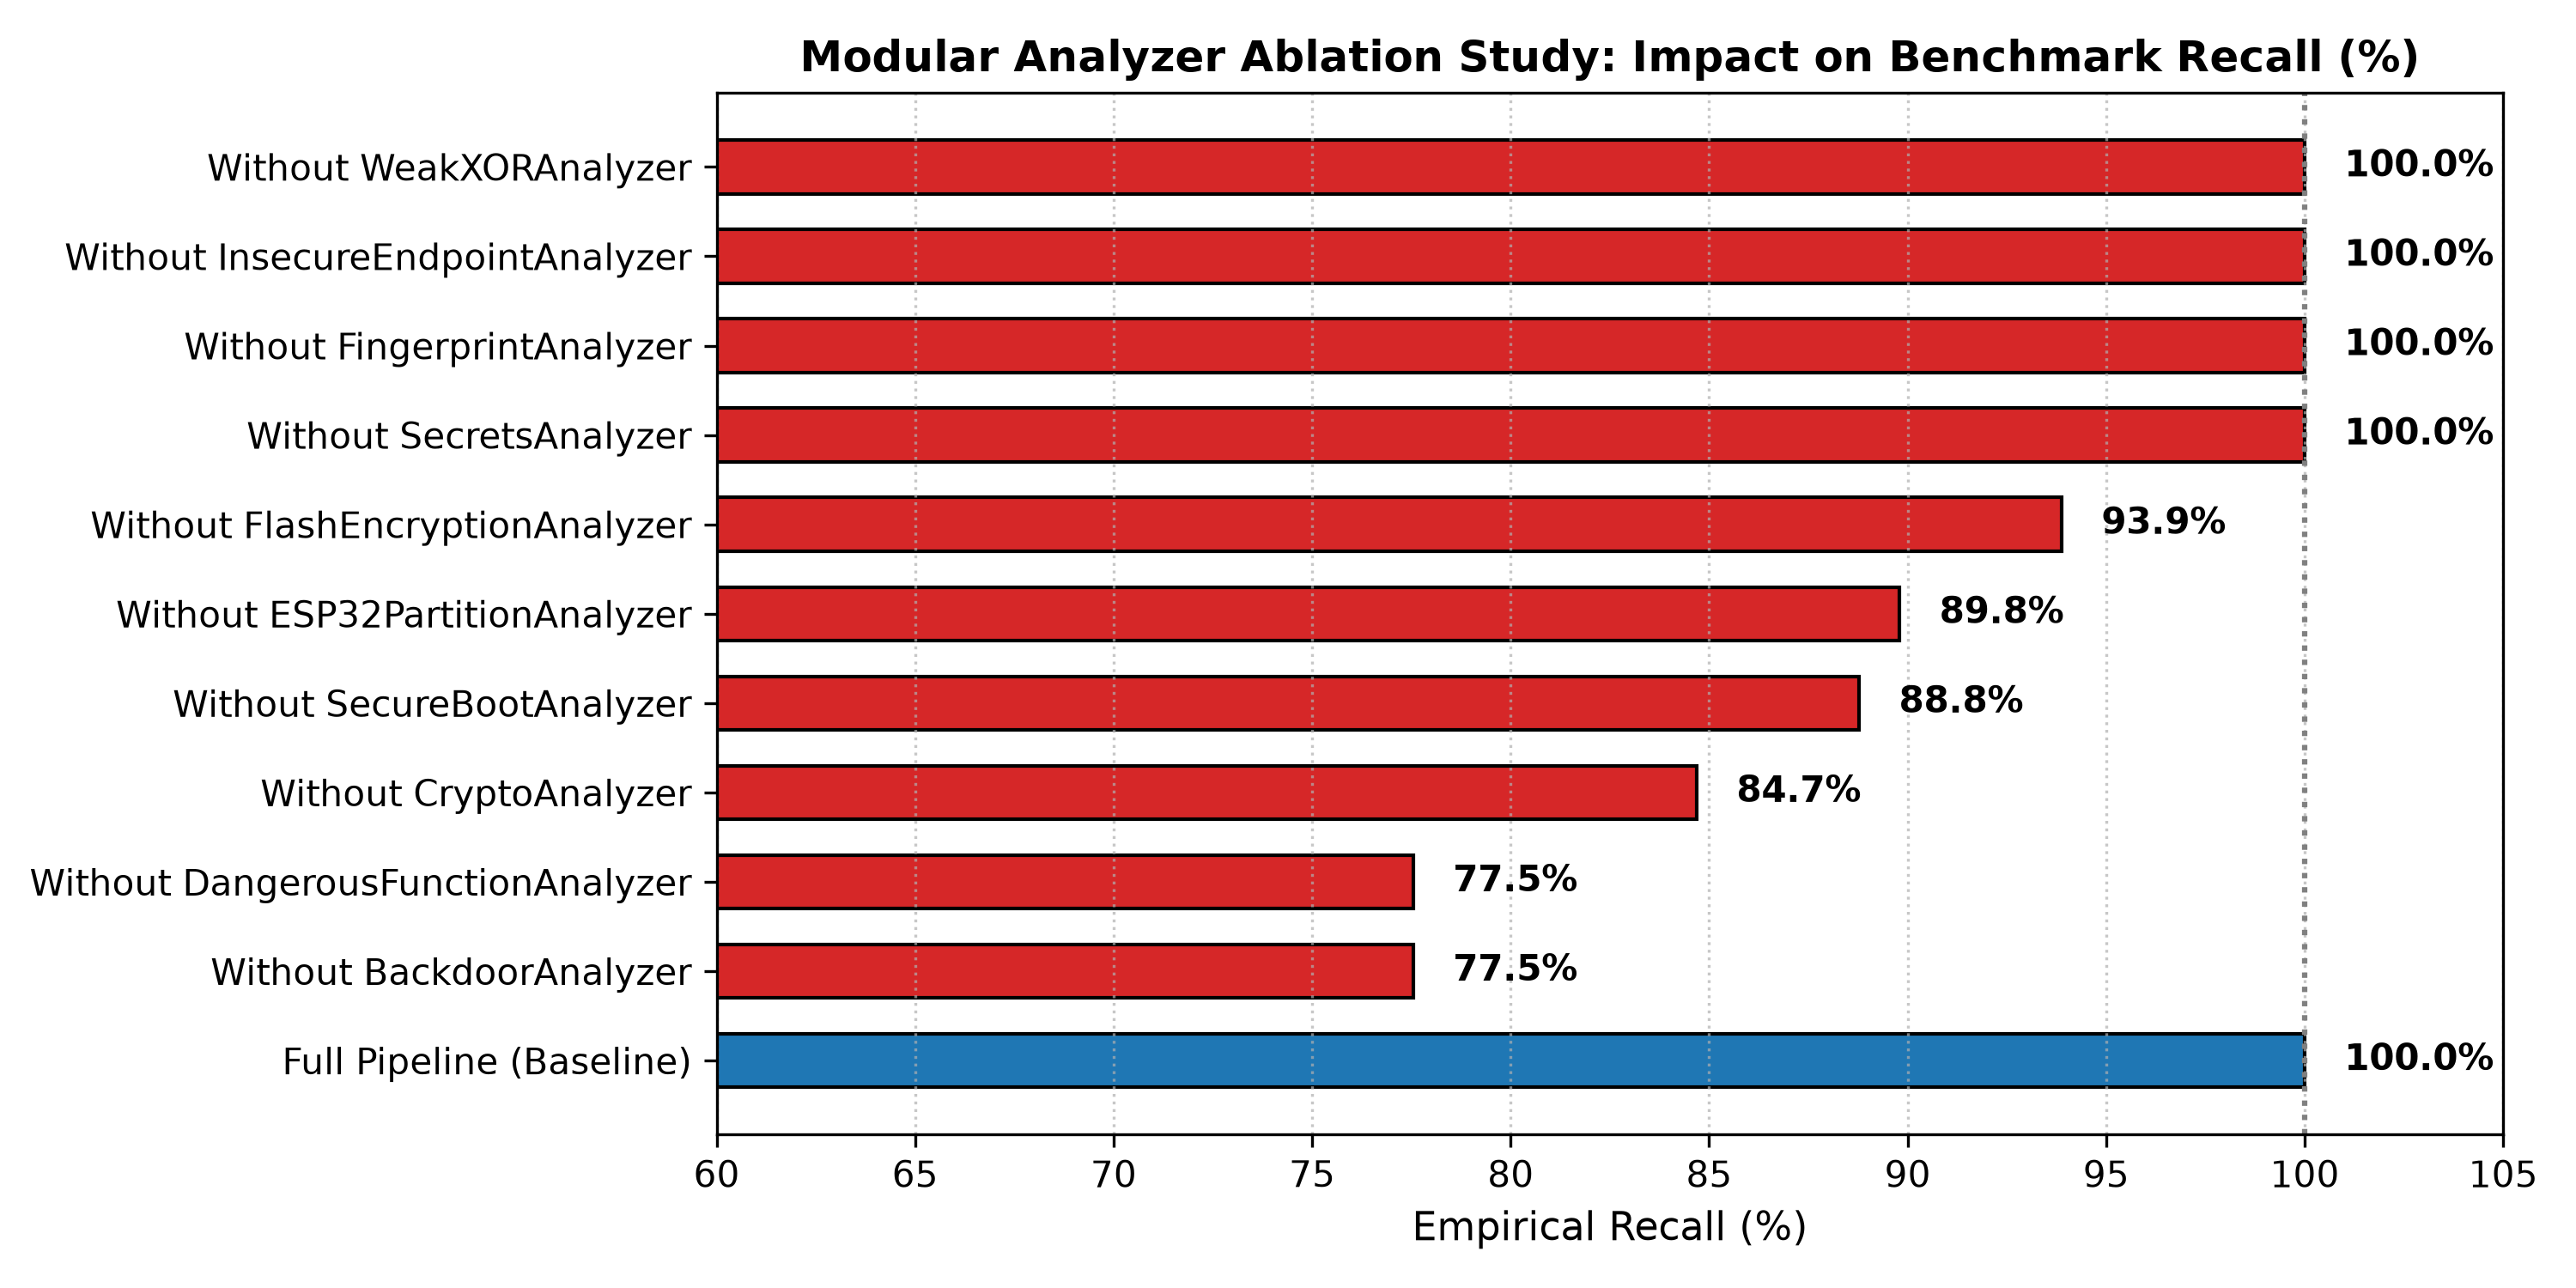
\includegraphics[width=0.92\columnwidth]{fig_ablation_recall.png}
\caption{Benchmark recall degradation under modular ablation.}
\label{fig:ablation_fig}
\end{figure}

Disabling \texttt{DangerousFunc} or \texttt{BackdoorAnalyzer} causes the most significant recall degradation ($\Delta$ -22.45\%). Ablating \texttt{CryptoAnalyzer} reduces recall by 15.31\%; notably, this drop is partially mitigated by overlapping CWE-327 detections from the \texttt{WeakXORAnalyzer}. Disabling \texttt{InsecureEndpointAnalyzer}, \texttt{SecretsAnalyzer}, or \texttt{WeakXORAnalyzer} maintains target CWE recall boundaries while removing large volumes of non-benchmark contextual findings (70, 64, and 7 findings respectively). \texttt{FingerprintAnalyzer} extracts platform compilation metadata and does not affect security metrics.

\subsection{Dynamic HIL Serial Validation}

Dynamic triage was evaluated on physical ESP32 hardware through UART at 115200\,baud. A five-case pilot test was used to exercise panic and fault-reporting behavior. The reproducible HIL evaluation did not establish the previously reported separation between four vulnerable cases and one clean control; therefore, no precision, recall, or F1 score is claimed for the HIL pilot. The experiment instead demonstrates the operational ability of the FirmLens serial monitor and crash parser to ingest and classify UART fault telemetry from physical ESP32 execution.

\section{Comparison with Prior Art}

Table~\ref{tab:comparison} summarizes system capabilities against existing firmware analysis frameworks.

\begin{table}[htbp]
\caption{System Capability Comparison with Existing Frameworks}
\label{tab:comparison}
\centering
\scriptsize
\setlength{\tabcolsep}{2.2pt}
\begin{tabularx}{\columnwidth}{@{}Xcccc@{}}
\toprule
\textbf{Target Capability} & \textbf{Binwalk} & \textbf{Firmadyne} & \textbf{EMBA} & \textbf{FirmLens} \\
\midrule
Bare-Metal RTOS Support    & No       & No       & No      & \textbf{Yes} \\
ESP32 Partition Parsing    & No       & No       & No      & \textbf{Yes} \\
Bootloader Crypto Audit    & No       & No       & Partial & \textbf{Yes} \\
Dynamic UART HIL Triage    & No       & No       & No      & \textbf{Yes} \\
Threat Intel Enrichment    & No       & No       & Partial & \textbf{Yes} \\
Sub-Second Static Scan     & Yes      & No       & No      & \textbf{Yes} \\
\bottomrule
\end{tabularx}
\end{table}

\section{Threats to Validity \& Limitations}
\label{sec:threats}

\begin{enumerate}

    \item \textbf{Construct Validity \& Synthetic Ground Truth}: Ground truth was formulated against representative ESP-IDF partition structures, known target characteristics, and synthetic CWE test vectors. The 100\% recall rate reflects agreement with the defined benchmark labels; it should not be interpreted as evidence of perfect detection on arbitrary or previously unseen firmware. Heavily obfuscated binaries, non-standard custom bootloaders, or vulnerabilities not represented by the benchmark may reduce static recall.

    \item \textbf{Dynamic HIL Pilot Scale}: Dynamic triage was evaluated using a five-case physical-hardware pilot over UART. The current reproducible run does not provide sufficient evidence for a quantitative vulnerable-versus-clean classification metric, so the HIL experiment is treated as operational validation rather than a statistically meaningful detection benchmark. Larger hardware cohorts and independently controlled fault injections are required for quantitative HIL evaluation.

    \item \textbf{Performance Measurement Environment}: Performance measurements were obtained on a macOS arm64 host with Python 3.14.6, 10 CPU cores, and 16\,GB RAM. Runtime and memory characteristics may differ across operating systems, processor architectures, Python versions, and system loads.

    \item \textbf{Architectural Scope}: FirmLens specializes in Espressif Xtensa and RISC-V targets. Adapting partition carving to ARM Cortex-M or MIPS microcontrollers requires target-specific partition and vector-table parsers.

\end{enumerate}

\section{Conclusion}

FirmLens presents an automated, low-latency security evaluation framework designed for bare-metal ESP32 microcontrollers. By uniting semantic partition parsing, hardware boot cryptographic auditing, threat intelligence correlation, and physical HIL panic classification, FirmLens provides a reproducible methodology for embedded firmware analysis. Evaluation across 11 benchmark targets achieved 95.15\% precision and 100.0\% recall against defined CWE ground truth, while modular ablation experiments quantified the contribution of individual analyzers. Physical HIL testing further demonstrated the crash parser's ability to process UART fault telemetry, while the limited pilot scale highlights the need for larger independently controlled hardware experiments.
  
\bibliographystyle{IEEEtran}
\bibliography{references}

\end{document}